\documentclass[9pt]{article}

\usepackage{lipsum}
\usepackage{graphicx}
\usepackage{amsmath}

\usepackage{etoolbox}
\usepackage[onehalfspacing]{setspace}
\AtBeginEnvironment{figure}{\singlespacing}
\AtBeginEnvironment{table}{\singlespacing}

\usepackage{caption}
\DeclareCaptionFont{8pt}{\fontsize{8pt}{9pt}\selectfont}
\captionsetup{font={8pt}}


\usepackage[
	backend=biber,
    style=authoryear,
    %sorting=ynt,
    bibwarn=true,
    bibencoding=utf8,
    sortlocale=de_DE,
    maxbibnames=99,
    maxcitenames=1]{biblatex}
    
\DefineBibliographyStrings{english}{
   andothers = {{et\,al\adddot}},}
   
\addbibresource{../../../bib/thesis.bib}

\AtBeginEnvironment{figure}{\singlespacing}
\AtBeginEnvironment{table}{\singlespacing}


\begin{document}


\begin{titlepage}
	\centering
	{\scshape\LARGE Ludwig-Maximilians-Universität München \par}
	{\scshape\large Department Biologie II Computational Neuroscience \par}
	\vspace{0.5cm}
	\includegraphics[width=0.7\textwidth]{../logo/GSN-Logo_ab35mmBreite_RGB.jpg}\par
	\includegraphics[width=0.4\textwidth]{../logo/siegel_black.pdf}\par
	\vspace{0.7cm}
	{\scshape\LARGE Report \par}
	\vspace{0.05cm}
	{\huge\bfseries Computational Simulation of Time Perception: Model Description and Implementation \par}
	\vspace{1.1cm}
	{\Large Katharina \textsc{Bracher} \par}
	{Student ID: 11754625 \par}
	\vspace{0.4cm}
	{\large Supervision: Dr. Kay \textsc{Thurley} \par}
\end{titlepage}


\normalsize
\tableofcontents
\pagebreak


\section{Behavioral Effects in Magnitude Estimation}
Magnitude estimation is subject to noise that arises from external sources i.e. the statistics of the environment and internal sources i.e. neural representation of the input and the behavior.
Across sensory modalities, characteristic behavioral effects are identified (\cite{Petzschner2015}).
The most prominent observation is a regression to the mean of the stimulus range,  i.e. small stimuli are overestimated whereas large stimuli are underestimated (\textit{regression effect}). 
This effect intensifies for ranges with larger stimuli (\textit{range effect})
For larger stimuli the standard deviation of estimates increases monotonically (\textit{scalar variability}). 
Finally, the recent history of stimuli presentations influences the current stimuli estimation (\textit{sequential effect}).
All effects mentioned above are displayed in Fig. \ref{fig:behavioraleffects}. 

Modality-independence of these effects suggests the existence of a common underlying principle or processing mechanisms, that would explain e.g. a optimal strategy for unreliable judgments due to noise (in stimuli and estimates).

\begin{figure}[ht]
	\centering
	\includegraphics{figures/behavioural_effects_petzschner.pdf}
	\caption{\textbf{Behavioral Effects} 
	\textit{Regression effect}: in a range of stimuli large stimuli are underestimated, and small stimuli are overestimated which results in a regression to the mean of the range.
	\textit{Range effect}: the regression to the mean gets more pronounced for ranges that comprise larger stimuli. 
	\textit{Scalar variability}: the standard deviation of the reproduced magnitude grows linearly with larger rages. 
	\textit{sequential effects}: the history presented stimuli (e.g. ascending or descending order) has an influence on the reproduced magnitude. 
	Adapted from \cite{Petzschner2015}.}
	\label{fig:behavioraleffects}
\end{figure}

During time perception and time reproduction experiments, neural activity displays characteristic trajectories in a low-dimensional space (\cite{Meirhaeghe2021}, \cite{Wang2018}, \cite{Henke2021}). 
The neural trajectories are consistently influenced by prior beliefs. 
Flexible motor timing can be achieved by controlling the speed of neural dynamics (\cite{Sohn2019}, \cite{Wang2018}). 
Further, it has been found that neural activity in anticipation of a delayed response reaches a fixed threshold with rate inversely proportional to delay period \cite{Murakami2014}, \cite{Mita2009}).
\cite{Wang2018} proposed a potential neural mechanism for speed control and based on that \cite{Egger2020} developed a neural circuit model for sensorimotor timing.

\section{Model Description}
\subsection{Basic Circuit}
Flexible speed control can be achieved by a simple model consisting of three units, $u, v, y$ that represent population activity. 
The dynamics of $u, v$, and $y$ are defined as follows:
\begin{equation} \label{circuit}
	\begin{split}
	\tau\frac{du}{dt} & = -u + \theta(W_{uI}I - W_{uv}v + \eta_u) \\
	\tau\frac{dv}{dt} & = -v + \theta(W_{vI}I - W_{vu}v + \eta_v) \\
	\tau\frac{dy}{dt} & = -y + W_{yu}u - W_{yv}v + \eta_y
	\end{split}
\end{equation}
Two units, $u$ and $v$ receive a tonic symmetric input $I$ ($W_{uI}=W_{vI}=6$) and are mutually inhibiting each other ($W_{uv}=W_{vu}=6$). 
The inputs to $u$ and $v$ are governed by a sigmoidal activation function $\theta(x) = \frac{1}{1+exp(-x)}$.
y is the output unit and receives excitatory input from $u$ and inhibitory input from $v$ ($W_{yu}=W_{yv}=1$) which results in ramp-like activity.
All three units have a time constant $\tau = 100$. 
Stochastic synaptic inputs are modeled as independent white noise $\eta_u, \eta_v, \eta_y$ with standard deviation $\sigma$.
Initial conditions of $u, v$ and $y$ have been optimized for in \cite{Egger2020} and are set to $u_0=0.7 , v_0=0.2 , y_0=0.5$.

Depending on the input $I$, the system shows different dynamics. For low levels of $I$ (0$<$I$<$0.5) the system has three fixed points (2 stable, 1 unstable at $u=v$) and y ramps up faster the higher the input $I$. 
For intermediate values of $I$ (0.5$<$I$<$1) the system still shows three FP of the same sort and $y$ ramps up with a slope that is inversely proportional to the input $I$ (y ramps up slower the higher the input $I$, see schematic in Fig. \ref{fig:circuit}a, b). 
For high $I$ (1$<$I) the system has one stable fixed point (at $u=v$) and $y$ ramps down faster for higher $I$.
Thus, the speed at which the output $y$ evolves can be controlled by the input $I$ to $u$ and $v$ (Fig. \ref{fig:circuit})b) and determines the time interval after which y reaches a fixed threshold $y_0$. 
Reaching the threshold $y_0$ can be understood as movement initiation time in interval reproduction experiments and adjusting $I$ means reproducing longer or shorter intervals.
In this report, the intermediate input regime is explored. In this regime, higher a higher input $I$ results in a smaller slope of $y$, such that the threshold $y_0$ is reached after a longer interval.

\begin{figure}[ht]
	\centering
	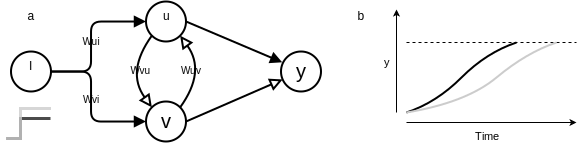
\includegraphics{figures/defCircuit.drawio.pdf}
	\caption{\textbf{Basic Circuit and Input Regimes} 
	\textbf{(a)} $u$ and $v$ share a common input $I$. Dynamics for example input $I=0.75$ in gray and $I=0.65$ in black plotted in (b). The input is governed by weights $W_{uI}$ and $W_{vI}$. The two units have reciprocal inhibitory connections with weights $W_{uv}$ and $W_{vu}$ that determine the inhibitory strength and project to the output unit $y$ with an excitatory connection from $u$ and an inhibitory connection from $v$. Excitatory and inhibitory connections are shown by filled and open arrows, respectively. 
	\textbf{(b)} Dynamics of $y$ for intermediate regime with input $I=0.75$ in gray and $I=0.65$ black. There is an inverse relation of input strength and slope. With higher input, the threshold at 0.7 (dashed line) is reached after a longer time interval. 
	\textbf{(c)} Dynamics of $u, v, y$ for inputs from $0.1\leq I \leq 1.5$ are shown. Initial conditions are set to $u_0=0.7 , v_0=0.2 , y_0=0.5$. With these initial conditions and values of $I>=0.5$, the relation of steady state activity of $y$ (and slope to reach steady state) is inverse to $I$ (intermediate and high I regime). For $I<0.5$ the steady state (slope) is smaller the smaller $I$ (low $I$ regime).}
\label{fig:circuit}
\end{figure}


\subsection{Update Mechanism and Experiment Procedure}

\begin{figure}
	\centering
	\includegraphics{figures/epochs.drawio.pdf}
	\caption{\textbf{Extended Circuit for Experiment Simulation} 
	\textbf{(a)} The circuits for measurement, reproduction and delay epoch is displayed. All circuits comprise the same basic structure with different additional elements that are unique for the epoch. Initial values of $u, v, y$ and $I$ are fed into the delay circuit for the initial duration. $u$ and $v$ are reset with $I_r$ before values of $u, v, y$ and $I$ are transferred to the measurement circuit. After the duration of the stimulus interval the difference between y and the threshold $y_0$ is used with the memory parameter $K$ to update $I$, that is, after another reset of $u$ and $v$, transferred with the other variables to the reproduction circuit. The reproduction ends when $y$ reaches the threshold $y_0$ from below. Before another stimulus interval, the reset values are fed into the delay circuit again for a fixed duration. The model is able to simulate an arbitrary number of stimulus intervals. Adapted from \cite{Petzschner2015}.
	\textbf{(b)} Interval reproduction experiment with stimulus interval $t_s$ (blue) and reproduction $t_r$ (red).
	\textbf{(c)} Schematic of a trial with one stimulus interval. After a delay epoch $u$ and $v$ are reset. The measurement epoch lasts for the duration of the stimulus interval. $y$ should reach the threshold $y_0$ (dashed line) at exactly the time the stimulus interval ends. The threshold was crossed well before the end of the interval and at the end of the measurement epoch, the error in $y_m$ to the threshold $y_0$ is used to update $I$. To reach the threshold at a later time $I$ is increased, which reduced the slope of $y$. After the reset of $u$ and $y$ and the update of $I$ the reproduction ends when $y$ reaches the threshold.}
\label{fig:epochs}
\end{figure}

For simulating time reproduction experiments, the relation of the input $I$ with the slope of the ramping activity of $y$ in combination with a fixed threshold $y_0$ is used.
Measuring and reproducing an interval is done predicatively, by adjusting the slope of the ramp such that the output reaches the threshold after the intended time. In other scenarios, time could be encoded by the level a ramp with a fixed slope reaches. 
By adding an update mechanism that can flexible adjust $I$, the threshold crossing of $y$ can be delayed or moved to earlier times.

Interval reproduction experiments can be designed with only two epochs. A measurement epoch that has the duration of the stimulus interval and a reproduction epoch that starts immediately after the measurement epoch (Fig. \ref{fig:epochs}b). 
The basic circuit is modified to perform interval reproduction (see figure \ref{fig:epochs}a for schematic of modified circuit).
In the model the measurement epoch is fixed, and the reproduction epoch ends, when y reaches the fixed threshold $y_0$ from below. 
The interval from the end of the measurement epoch and the threshold-crossing of $y$ yields the reproduced time that is aimed to equal the stimulus interval that was presented as measurement epoch (Fig. \ref{fig:epochs}c).

The following update mechanism of $I$ is based on the intermediate regime of $I$, that shows an inverse relation of $I$ to the slope of $y$ (Fig. \ref{fig:circuit}b).
The error signal is determined at the end of the measurement epoch and is composed of the difference of $y$ to the threshold $y_0$.
If the threshold $y_0$ is not reached during the measurement epoch, the slope has to be adjusted, such that y ramps up faster to reach the threshold at exactly the time of the stimulus interval. For a steeper slope, $I$ is reduced.
If $y$ crossed the threshold before the measurement epoch ends, so is above $y_0$ by the end of the stimulus interval, the slope needs to be reduced in order to reach the threshold at a later time in the reproduction. For a shallower slope, $I$ is increased.
Adjusting $I$ is done by the difference of $(y-y_0)$, weighted by a memory parameter $K$ right at the end of the measurement epoch.
\begin{equation} \label{Iupdate}
	\begin{split}
	\tau\frac{dI}{dt} & = sK(y-y_0)
	\end{split}
\end{equation}
The update of $I$ is only active for a pulse between the measurement and reproduction epoch ($s=1$) and inactive for all other times ($s=0$).
Further, $u$ and $v$ are reset by a transient input $I_r$ pulse to reset the dynamics for the subsequent epoch (Fig. \ref{fig:epochs}c).
\begin{equation} \label{experimentcircuit}
	\begin{split}
	\tau\frac{du}{dt} & = -u + \theta(W_{uI}I - W_{uv}v + \eta_u - I_r) \\
	\tau\frac{dv}{dt} & = -v + \theta(W_{vI}I - W_{vu}v + \eta_v + I_r) \\
	\end{split}
\end{equation}
Resetting the dynamics after the reproduction epoch enables the model to simulate an arbitrary number of stimulus intervals. 
Before a new stimulus presentation in the measurement there is a delay period and in the beginning of a trial there is an initial interval that starts with the initial values of $u, v, y$ and an initial input $I_0$ (Fig. \ref{fig:epochs}c). 
The additional interval in the beginning of a trial allows the model to get closer to steady-state before the stimulus presentation starts. 
Reproductions that do not reach the threshold in a certain time span (twice the stimulus interval) are classified as timeout trials. 
If the threshold is crossed particularly early, the trial is also classified as (early) timeout trial (crossing before 0.2 of stimulus interval).
To simulate variability in the reproductions as it is found in real data, noise is added to $u, v$ and $y$ in the implementation. In data an monotonic increase of the standard deviation of reproductions is found (\textit{scalar variability}). 
If noise levels in the model are too high ($\sigma>0.25*I$) the standard deviation of reproductions is not growing monotonically with $\sigma$ (\cite{Egger2020}). 
For an example trial see figure \ref{fig:trial}. 

\begin{figure}[ht]
	\centering
	\includegraphics{figures/trial.drawio.pdf}
	\caption{\textbf{Experiment Simulation} Example trial with 5 stimulus intervals (700, 500, 600, 700, 600 ms). Initial values are set to $u_0=0.7 , v_0=0.2 , y_0=0.5. I_0=0.8$) other parameters are $\sigma=0.01$, the initial duration of 750 ms and a 700 ms delay period before new stimuli. The dynamics of $u, v, y $ and $I$ are displayed over time. The threshold is set to $y_0=0.7$ (dashed line). The first stimulus interval is reproduced poorly as the system needs more trials to adapt the initial $I_0$ to a suitable range (reproduced times 1040, 650, 530, 620, 570 ms).}
\label{fig:trial}
\end{figure}


\section{Implementation of the Model}
All simulations and analysis was performed with Python 3.9.7. 
For simulating the dynamics Euler's method was used. The step size $\Delta t$ was set to 10 ms.
The reset mechanism of $u$ and $v$ is switched on for one time step after every epoch and the update mechanism of $I$ is switched on for one time step after the measurement epoch only. 
Noise is independently sampled for every time step from a Gaussian distribution with standard deviation $\sigma$
Definition of timeouts


\section{Supplements}

\subsection{Code}
\begin{figure}[ht]
	\makebox[\textwidth][c]{\includegraphics[width=1.2\textwidth]{figures/codeStructure.drawio.pdf}}
	\caption{\textbf{Code Structure}}
\label{fig:code}
\end{figure}

The code consists of a Base Simulation with the Euler implementation of the dynamics of $u, v, y$ and $I$. Each epoch or pulse between epochs is fed into the network in BaseSimulation and results are added to the course of the trial in trial\_update. 
Two kinds of experiments are implemented. An interval reproduction experiment, as described in this report is implements in experiment\_simulation. 
Parallel simulations of one run (delay, measurement, reproduction epoch) is implemented in parallel\_simulation. Both rely on BaseSimulation (for overview of classes see figure \ref{fig:code})



\printbibliography

\end{document}